\section{Исследование и построение решения задачи}
\label{sec:research_and_solving} \index{research_and_solving}
\subsection{Описание предложенного решения задачи}
В этом разделе будет описаны методы построения представления сложноструктурированных событий, рассмотрена интерпретируемость каждого из представлений, и показано, какие методы можно использовать для решения  непосредственно задачи прогнозирования.

\subsubsection{Построение представления событий}
\label{subsub:repr}
% PCA
% NMF Неотрицательная факторизация матрицы
% AE Нейросетевой автокодировщик
При построении представления сложноструктурированных событий и с учетом их временной неравномерности,
мы требуем от такого представления возможность агрегации по времени. Также для неявного (скрытого) представления событий хотелось бы иметь возможность его интерпретации, чтобы можно было производить какой-то анализ как самого представления, так и использующих его моделей.

Перед переходом к построению представления, опишем предлагаемые методы обработки различных типов признаков.
Числовые и бинарные признаки не предобрабатывались, категориальные признаки переводились в бинарные с помощью унитарного кодирования (one-hot encoding). Для категориальных признаков также можно использовать любой метод перевода их в бинарные/числовые признаки: кодирование уникальными значениями и другие.
Текстовые описания можно преобразовать в числовые вектора одним из многих способов: латентным размещение Дирихле (LDA), кодированием tf-idf или нейросетевыми моделями (word2vec, doc2vec, скрытое представление с помощью LSTM). В этой работе я использовал латентное размещение Дирихле для предобработки текстовых данных. После такой обработки все признаки становятся либо числовыми, либо бинарными.

Несмотря на то, что числовые и бинарные признаки обладают возможностью агрегации по времени, велика вероятность того, что они избыточны, а значит можно найти такое представление, которое переведет исходные признаки в пространство меньшей размерности и будет более уместно для использования в задаче прогнозирования. 

В качестве базового подхода были рассмотрены такие методы понижения размерности как Метод главных компонент (PCA \cite{pca_orig}), Неотрицательная факторизация матриц (NMF \cite{nmf_orig}). В этой работе было решено остановиться на более тщательном исследовании применимости неотрицательной факторизации матриц. 

Общая идея факторизации матрицы заключается в следующем: 
Пусть $n$ -- количество событий, $d$ -- размерность вектора признаков каждого события. Обозначим исходную матрицу описывающую события как $V$, $V \in \mathbf{R}^{n \times d}$. Задача факторизация матрицы $V$ заключается в нахождении матриц $W \in \mathbf{R}^{n \times k}, H \in \mathbf{R}^{k \times d}$, $k \ll d$ таких, что эти матрицы $W, H$ минимизируют $||V - W \cdot H||$. Из такого разложения видно, что матрица $H$ показывает соотношение между исходными $n$ признаками и новыми $k$ признаками. Эти новые $k$ признаков мы будем в дальнейшем называть тематиками или скрытыми (латентными) признаками. Также будем называть матрицу $W$ матрицей \textit{событий-тематик}, а матрицу $H$ матрицей \textit{тематик-признаков}.
При использовании неотрицательной факторизации матрицы, тематики представляют из себя линейные комбинации исходных признаков с неотрицательными весами, что делает интерпретируемость этих тематик тривиальной задачей.

Процесс факторизации является итеративным, в начале матрицы $W, H$ инициализируются неотрицательными значениями, затем они поочередно обновляются следующим образом:
$$H^{n+1}_{[i,j]} = H^n_{[i,j]} \frac{((W_n)^TV)_{[i,j]}}{((W^n)^TW^nH^n)_{i,j]}}$$
$$W^{n+1}_{[i,j]} = W^n_{[i,j]} \frac{(V(H^{n+1})^T)_{[i,j]}}{(W^nH^{n+1}(H^{n+1})^T)_{[i,j]}}$$

После того, как процесс сойдется, мы получаем матрицы $W,H$.

В качестве более продвинутого метода построения представления событий будет рассмотрен глубокий нейросетевой автокодировщик (далее -- просто автокодировщик) \cite{ae_orig}. 
Автокодировщик это специальная архитектура искусственных нейронных сетей, позволяющая применять обучение без учителя при использовании метода обратного распространения ошибки.

Простейшая архитектура автокодировщика — сеть прямого распространения, схожая с многослойным перцептроном и содержащая блок слоев для перевода входного вектора в скрытый код (кодировщик) и блок слоев для перевода скрытого кода в выходной вектор (декодировщик). В отличие от стандартных нейросетевых архитектур, выходной слой автокодировщика содержит столько же нейронов, сколько и входной слой, а задачей всей сети является перевод входного вектора в код меньшей размерности (кодировщик) и дальнейшее восстановление вектора из его кода с минимизацией ошибки восстановления (декодировщик). Пример архитектуры однослойного автокодировщика представлен на Рис. \ref{fig:ae_arch}.
\begin{figure}
\centering
  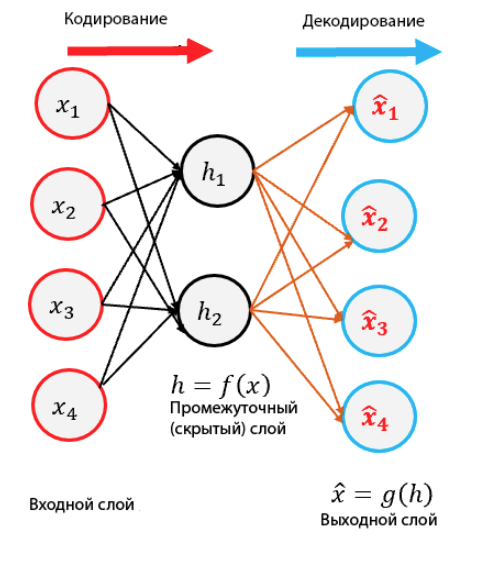
\includegraphics[width=.4\linewidth]{ae_arch_ru.png}
  \caption{Пример архитектуры простого автокодировщика}
  \label{fig:ae_arch}
\end{figure}

Более формально, автокодировщик нелинейно преобразует входной вектор $x \in \mathbf{R}^d$ в $z \in \mathbf{R}^k$, а затем производит реконструкцию вектора $x$ используя $z$. В результате реконструкции получается вектор $x' \in \mathbf{R}^d$, и задача автокодировщика -- минимизировать ошибку восстановления $L(x,x')$ (например $L(x,x')=||x - x'||$).

После обучения модели с такой архитектурой, можно использовать только ее первую часть (кодировщик) для получения $z^*$ их произвольного входного вектора $x^*$ и использовать этот код $z^*$ как скрытое представление события. В таком случае скрытыми тематиками будем называть элементы вектора $z^*$.
Так как преобразования кодировщика нелинейны, интерпретация скрытого кода затруднительна, эта проблема будет рассмотрена отдельно в следующем разделе.

% Auxiliary features
В процессе исследования решения задачи, было решено добавить два дополнительных признака для выделения более явной регрессионной компоненты. Для каждого агрегационного периода вычислялось:
\begin{enumerate}
   \item $N_{all}$, общее количество событий, входящих в этот период
   \item $N_{target}$, количество целевых событий, входящих в этот период
\end{enumerate}

Эти признаки можно было бы назвать ''экспертными'' или ''созданными вручную'', но они не умаляют общности подхода, так как применимы для задачи прогнозирования событий в целом.

% Recon features
Также вместе с признаками, полученными с помощью автокодировщика было предложено использовать в качестве дополнительного признака ошибку восстановления автокодировщика (т.е. признак, показывающий, насколько восстановленный автокодировщиком вектор признаков отличается от исходного вектора признаков):

$recon\_err = x' - x$, следуя нотации введенной ранее.

Мотивация добавления подобного признака следует из области выявления аномалий \cite{anomaly_detection_ae} и заключается в следующем: если исходный вектор признаков сильно отличается от восстановленного вектора признаков (большая ошибка восстановления), то есть основания полагать, что этот вектор является в некотором смысле аномальным и модель с помощью значения такого признака сможет учитывать аномальность конкретного события.

\subsubsection{Интерпретируемость представления}
\label{subsub:interp}
Как было сказано выше, важной характеристикой скрытого представления событий является его интерпретируемость. Если у представления такое свойство есть, то становится возможным анализ полученных тематик, а так же анализ результатов прогнозирования и их более глубокое понимание.

По своей природе скрытые признаки, выделенные неотрицательной факторизацией матриц и методом главных компонент интерпретируемы, поскольку эти скрытые признаки представляют собой линейные комбинации исходных признаков. В случае неотрицательной факторизацией матриц, если рассмотреть вышеупомянутую матрицу \textit{тематик-признаков}, можно увидеть, что каждая тематика описывается набором неотрицательных весов, соответствующих оригинальным признакам. Чем больше вес у некоторого признака, тем более сильный вклад этот признак вносит в данную тематику. 
Пример того, как можно описать одну из тематик, выделенных NMF, можно увидеть на Рис. \ref{fig:nmf_topic}. На этом рисунке изображены 9 исходных признаков с наибольшими весати, т.е. вносящих максимальный вклад в тематику.
\begin{figure}
  \centering
  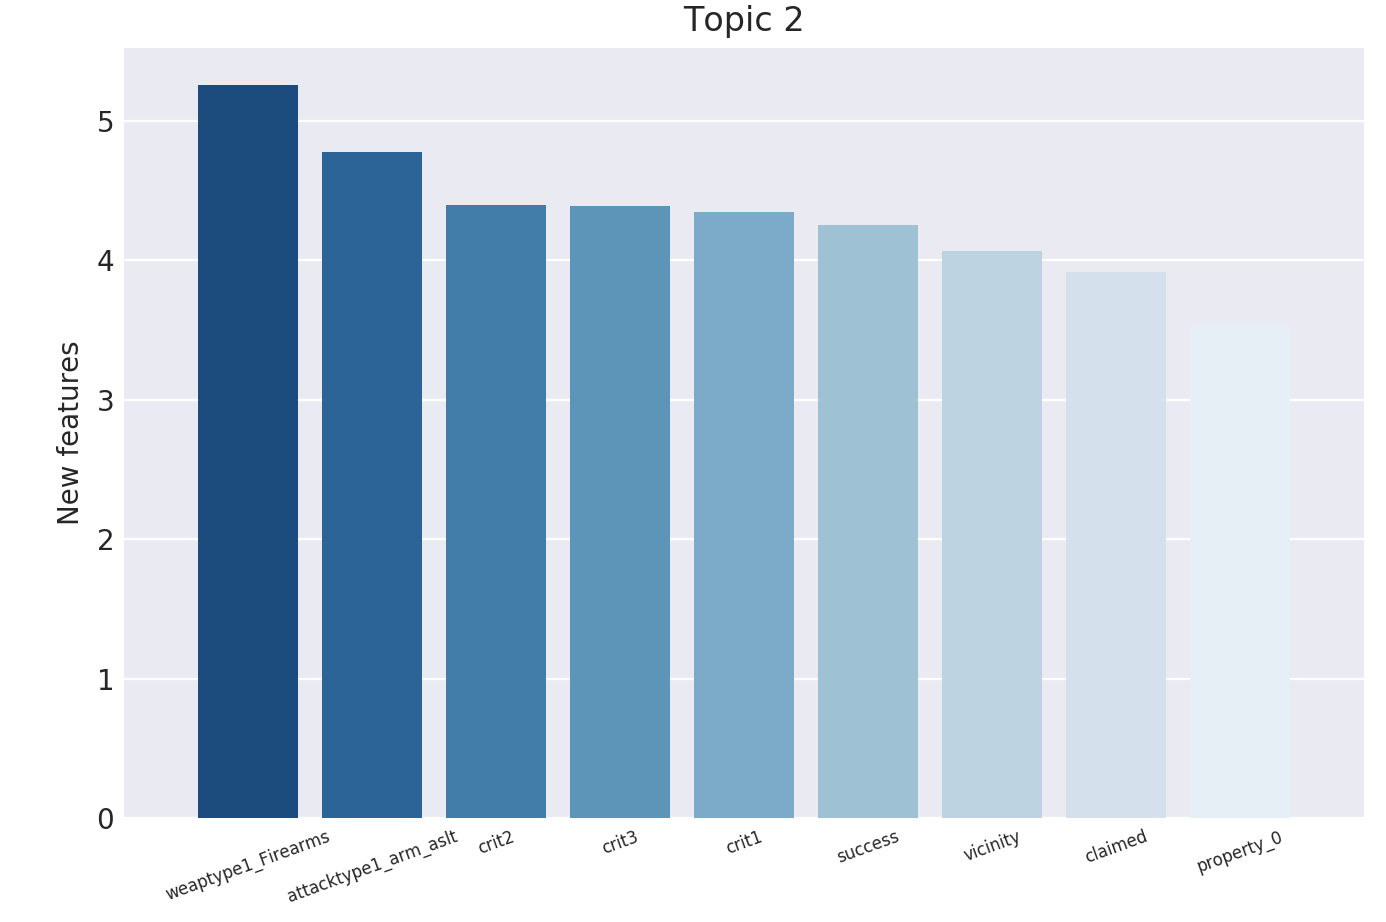
\includegraphics[width=.8\linewidth]{nmftopic.png}
  \caption{Пример интерпретации тематики, выделенной с помощью неотрицательной факторизации матриц}
  \label{fig:nmf_topic}
\end{figure}

В случае, когда преобразование исходного пространства признаков более сложное и нелинейное, необходимы другие методы интерпретации.
В данной работе предлагается метод, основанный на текстовых описаниях, доступных хотя бы для части событий.

Первый шаг получения интерпретации тематик это извлечь все доступные текстовые описания, обработать их стандартными методами (привести к нижнему регистру, убрать пунктуацию и стоп-слова, нормализовать формы слов) и составить словарь из полученного набора термов. Обозначим размер этого словаря как $n_w$.
Затем выберем из всего множества событий те, у которых есть текстовые описания, и каждому событию сопоставим $n_w$ бинарных признаков, показывающих вхождение или отсутствие каждого слова из словаря в текстовом описании этого события.

После составления таких признаков, для каждой тематики необходимо посчитать корреляции между значениями этой тематики и каждым из построенных бинарных признаков. И наконец можно получить для этой тематики описание из $k$ ключевых слов взяв для нее $k$ максимально кореллирующих с ней бинарных признаков.
Этот метод интерпретации в чем-то похож на тот, который мы применяли к неотрицательной матричной факторизации: чем сильнее корреляция, тем точнее можно описать тематику этим ключевым словом. Основное отличие этого метода -- он применим для интерпретации любого представления событий, единственное требование -- наличие текстовых описаний хотя бы у части из них. Как показали эксперименты, даже менее чем 20\% событий с текстовыми описаниями достаточно для построения описаний тематик.

Как дополнительный результат этого метода, можно получить описание любого события ключевыми словами, выбрав некоторое количество ключевых слов из описаний каждой тематики пропорционально значениям этих тематик у события.

\subsubsection{Прогнозирование событий}
% % classic: RF, LR, MachineLearning \subsubsectionЛогистическая/линейная регрессия (LogReg/LinReg)
% % NN: Модель с долгой краткосрочной памятью (LSTM}
\label{subsub:forecasting}
После того как получено подходящее представление событий, возникает вопрос об их прогнозировании. Для использования классических и хорошо изученных методов необходимо каждому событию сопоставить бинарную метку -- является ли оно интересующим нас событием.
Обозначим множество всех событий как  $E_{all}$, а множество интересующих нас событий как $E_{in}$. Тогда метка $y_e$ для события $e$ определяется следующим образом: $1$ если $e \in E_{in}$ и $0$ иначе.

В дальнейших рассуждениях будем подразумевать, что каждое событие $e$ имеет временную метку $t_e$ и набор значений тематик $x_e$ (т.е. представление события $e$, описывающее это событие).

После выбора размера интервала агрегации $\Delta t$, мы получаем разбиение временной шкалы на интервалы размера $\Delta t$. 
Для каждого такого интервала $T_i$ мы получаем усредненные значения тематик событий, принадлежащих этому интервалу.
$$\bar{x_i} = \frac{1}{|\{i: t_{e_i} \in T_i\}|} \sum_{\{i: t_{e_i} \in T_i\}}{x_{e_i}}$$ 

Агрегация меток событий производится в зависимости от решаемой задачи:
$$\bar{y_i} = \sum_{\{i: t_{e_i} \in T_i\}}{y_{e_i}},$$ для прогнозирования количества событий и

$$\bar{y_i} = max_{\{i: t_{e_i} \in T_i\}}{y_{e_i}}, $$ для прогнозирования вероятности события.

После выполнения указанных выше преобразований, мы получаем многомерный временной ряд, где значения $\bar{x}_{0,1,...}$ являются значениями этого ряда. 
Поскольку прогнозирование будет основываться на исторических данных, обозначим количество используемых предшествующих интервалов за $L$. С учетом этих обозначений, формально проблему прогнозирования можно описать как нахождение $\hat{y}_{i+1}$ при данных $\bar{x}_{i-L+1}, \bar{x}_{i-L+2}, ...,\bar{x}_{i}$, где $\hat{y}_{i+1}$ это предсказанное значение $\bar{y}_{i+1}$.

В данной работе предлагаются два различных подхода к такому прогнозированию. Первый и базовый подход -- объединить значения тематик с $L$ предшествующих интервалов в один вектор, опционально добавить дополнительные признаки предложенные выше и используя классические методы обучить на этих данных классификатор или регрессор, в зависимости от задачи.

%% TODO add LSTM 
Вторым подходом является использование нейросетевой архитектуры долгой краткосрочной памяти (Long short-term memory; LSTM) \cite{lstm_orig} .

Архитектура искусственных нейронных сетей LSTM основана на идее рекуррентных нейронных сетей (RNN). Рекуррентные нейронный сети -- семейство нейронных сетей, в которых связи между узлами формируют направленную последовательность. Также у рекуррентных нейронных сетей есть внутреннее состояние  (память), с помощью которого такие сети могут работать с входными последовательностями различной длины. Основной недостаток данной архитектуры -- проблемы с градиентами при работе алгоритма обратного распространения ошибки по времени (т.е. по элементам последовательности в обратном порядке). В случае, если последовательность достаточно длинная, может возникнуть проблема исчезающих градиентов, при которой градиенты из-за очень долгого пути и большого числа умножений на матрицы вырождаются в 0 и веса нейронной сети перестают обновляться. Другая и прямо противоположная проблема -- проблема зашкаливания градиентов, при которой, опять же из-за длинного пути градиентов и большого количества умножений градиенты неконтролируемо и очень быстро растут, стремительно превышая разумные пределы. Нейросетевая архитектура долгой краткосрочной памяти призвана решить обе эти проблемы, в ней на каждой итерации (т.е. при обработке каждого нового элемента последовательности) происходит не просто умножение входных данных на матрицу, а обработка этих данных более сложным блоком. Блок содержит в себе \textit{ячейку памяти} и 3 \textit{вентиля}: \textit{входной вентиль}, \textit{выходной вентиль} и \textit{вентиль забывания}. 

Ячейка памяти в сетях долгой краткосрочной памяти интуитивно позволяет запоминать информацию о зависимостях между элементами последовательности. Входной вентиль контролирует то, какая часть входных данных (нового элемента последовательности) будет учитываться при дальнейших вычислениях в блоке. Выходной вентиль контролирует, какая часть информации из ячейки памяти будет использована для вычислений выходного сигнала блока. Вентиль забывания определяет, какая часть данных из памяти сохранится при переходе на следующий шаг, а какая часть будет удалена (забыта). Ключевой особенностью этой архитектуры является то, что благодаря ячейке памяти и структуре блока градиент не исчезает при использовании метода обратного распространения ошибки во времени. Иллюстрация архитектуры блока показана на рис. \ref{fig:lstm_arch}, а вычисления внутри блока производятся следующим образом:\\
$f_t = \sigma_g(W_{f} x_t + U_{f} h_{t-1} + b_f)$ \\
$i_t = \sigma_g(W_{i} x_t + U_{i} h_{t-1} + b_i)$ \\
$o_t = \sigma_g(W_{o} x_t + U_{o} h_{t-1} + b_o)$ \\
$c_t = f_t \circ c_{t-1} + i_t \circ \sigma_c(W_{c} x_t + U_{c} h_{t-1} + b_c)$ \\
$h_t = o_t \circ \sigma_h(c_t),$ \\
где \\
$x_{t}x_t$ — входной вектор,\\
$h_{t}$ — выходной вектор,\\
$c_{t}$ — вектор состояний,\\
$W,\ U$ и $b$ — матрицы параметров и вектор,\\
$f_{t},\ i_{t}$ и $o_{t}$ — векторы вентилей:\\
$f_{t}$ — вектор вентиля забывания, вес запоминания старой информации,\\
$i_{t}$ — вектор входного вентиля, вес получения новой информации,\\
$o_{t}$ — вектор выходного вентиля, кандидат на выход.\\
В формулах выше используются следующие функции: \\
$\sigma_{g}$: функция активации на основе сигмоиды.\\
$\sigma_{c}, \sigma_{h}$: функция активации на основе гиперболического тангенса.\\
$\circ$: произведение Адамара или покомпонентное произведение.

\begin{figure}
  \centering
  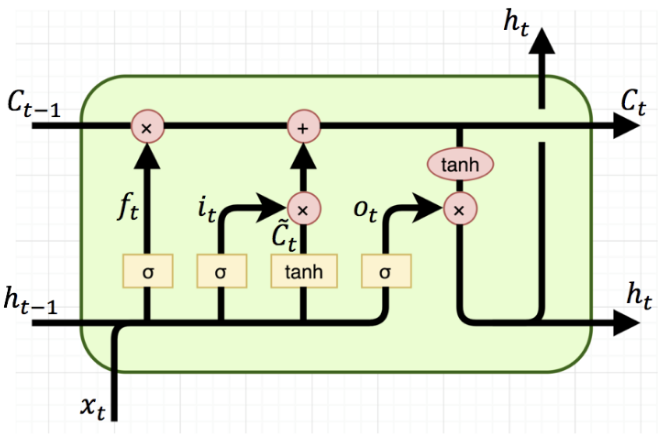
\includegraphics[width=.7\linewidth]{images/lstm_arch.png}
  \caption{Архитектура блока LSTM. $f_t,\ i_t,\ o_t$ - вентили забывания, входа и выхода. $x_t$ -- входной сигнал, $h_t$ -- выходной сигнал и внутреннее состояние блока. $C_t,\ C_{t-1}$ -- состояния ячейки памяти на $t$-м и $t-1$-м шагах соответственно}
  \label{fig:lstm_arch}
\end{figure}


В случае использования сети долгой краткосрочной памяти $L$ векторов будут последовательно поданы на вход модели, начиная с  $\bar{x}_{i-L+1}$ и заканчивая $\bar{x}_{i}$, а на выходе модель будет выдавать прогноз $\hat{y}_{i+1}$. При обучении модель будет пытаться обеспечить на последнем слое такой вывод $\hat{y}_{i+1}$, который был бы максимально похож на прогнозируемое значение $\bar{y}_{i+1}$.

\subsection{Экспериментальная часть}
Для экспериментальной оценки реализации предложенного решения мы использовали набор данных GTD\_0616 \cite{db:gtd}.
% GTD description
Этот набор данных обладает следующими особенностями:
	\begin{enumerate}
		\item Содержит подробную информацию о терактах начиная с 1975 года
		\item Содержит 55'600 записей с 1991 по 2012 год
        \item Информация включает в себя подробное описание теракта: дата, страна, группировка, ущерб, ...
        \item Содержит разнородные признаки: количественные, категориальные и, для некоторых событий, текстовые описания.
	\end{enumerate}

% Data aggregation using NMF model
\subsubsection{Построение представления событий и интерпретируемость}
Чтобы получить необходимое нам представление событий в пространстве тематик, были использованы алгоритм матричной факторизации NMF и нейросетевой подход, основанный на автокодировщиках.
После преобразований, описанных в начале раздела \ref{subsub:repr} и агрегирования мы перешли от отдельных событий к \textit{временному периоду}, содержащему некоторые события с помощью усреднения значений тематик для событий, входящих в этот период. Далее будем называть этот период \textit{агрегационным периодом} или просто \textit{периодом}. Затем к предобработанным данным мы применяли методы построения представления событий, пример 10 выделенных тематик как результат работы алгоритма неотрицательной факторизации матриц можно видеть на  Рис. \ref{fig:features_example}.

\begin{figure}
  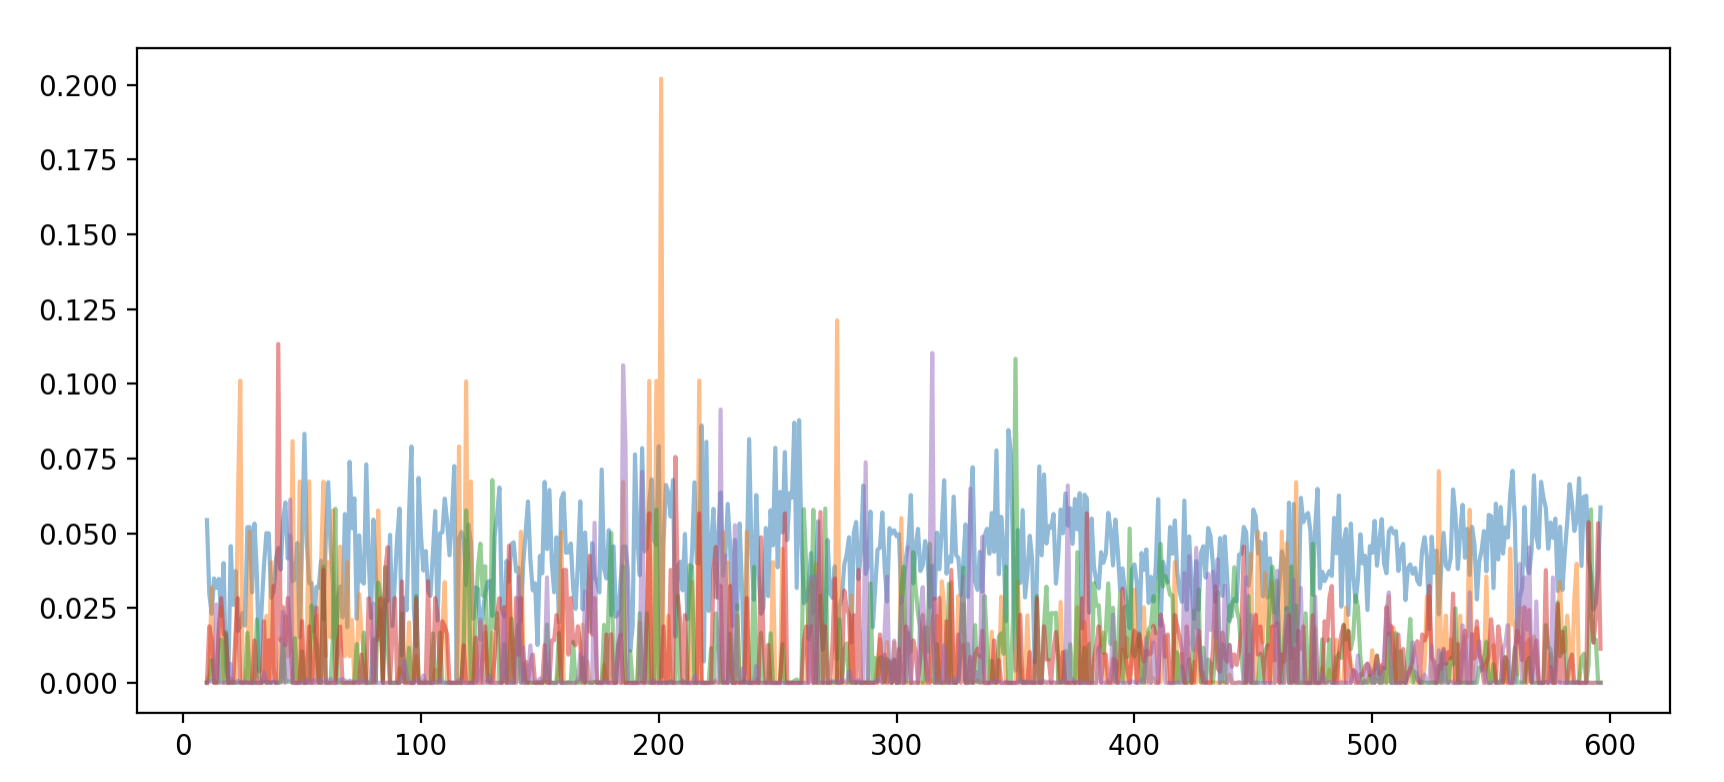
\includegraphics[width=\linewidth]{features_example.png}
  \caption{Пример временных рядов для тематик NMF}
  \label{fig:features_example}
\end{figure}

В случае с нейросетевым автокодировщиком, использовалась архитектура, описанная в таблице \ref{table:ae_arch}. Для кодировщика последовательно использовались полносвязные слои размерностей 256, 128 и 50 (размерность кода). Для декодировщика использовались полносвязные слои тех же размерностей, но в обратном порядке. Размерность входного вектора была равна 414, в рамках экспериментов были исследованы размерности скрытого кода равные 10 и 50. Для обучения модели применялась функция потерь $MAE$, описанная выше.
Количество эпох (т.е. количество проходов по всем имеющимся данным) при обучение модели было выбрано равным 100, начальный темп обучения был выбран равным  $2\cdot 10^{-3}$, также было использование экспоненциальное затухание темпа обучения: после каждой эпохи величина темпа обучения умножалась на 0.96.

\begin{table}
\centering
 \begin{tabular}{| c | c | c | c | c |} 
 \hline
 Название слоя & Тип слоя & Размер входа & Размер выхода & Функция активации\\
 \hline
 \hline
 кодировщик(1) & Полносвязный & 414 & 256 & ReLU\\ 
 \hline
 кодировщик(2) & Полносвязный & 256 & 128 & ReLU\\ 
 \hline
 кодировщик(3) & Полносвязный & 128 & 50 & ReLU\\ 
 \hline
 декодировщик(1) & Полносвязный & 50 & 128 & ReLU\\ 
 \hline
 декодировщик(2) & Полносвязный & 128 & 256 & ReLU\\ 
 \hline
 декодировщик(3) & Полносвязный & 256 & 414 & ReLU\\ 
 \hline
\end{tabular}
\caption{Архитектура автокодировщика}
\label{table:ae_arch}
\end{table}

Для интерпретации тематик методом, описанным в \ref{subsub:interp}, из набора данных были извлечены 19335 событий с текстовыми описаниями. После предобработки описаний и выделения слов был получен словарь размера 2311. После применения всей процедуры, описанной в \ref{subsub:interp} были получены наборы ключевых слов, описывающие тематики. Примеры таких ключевых слов для первых 5 тематик указаны в таблице \ref{table:kw_example}.

\begin{table}
\centering
 \begin{tabular}{c c} 
 \hline
 Тематика & Ключевые слова\\ 
 \hline
 \hline
 0 & used, sources, available, majority, listed, database, ...\\
 \hline
 1 & shot, civilian, distributed, bomb, detonated, ...\\
 \hline
 2 & taliban, shrine, perpetrators, tamil, rebels, group, ...\\
 \hline
 3 & released, hostage, kidnapping, status, abduction, ...\\
 \hline
 4 & indicated, military, police, civilian, detonating, ...\\
 \hline
 \end{tabular}
\caption{Примеры ключевых слов из описаний тематик }
\label{table:kw_example}
\end{table}


\subsubsection{Описание процесса обучения и тестирования} \label{train_process}
% NMF topics with lags as features
Метод прогнозирования, описываемый в моей работе, основывается на предположении, что вероятность наступления события (или количество событий) зависит от предшествующих событий, а точнее от значений тематик в агрегационных периодах, предшествующих периоду, для которого мы предсказываем эту вероятность.
В качестве признаков использовались значения тематик из $L$ предшествующих периодов, и таким образом для $k$ тематик размерность итогового пространства признаков становилась равна $L \cdot k$.

% target generation
Чтобы сформировать \textit{целевую переменную} необходимо было сначала определить события, которые нас интересуют (далее - \textit{целевые события}), в этой работе такие события определены как теракты, произошедшие в Ираке с типом атаки "взрыв". Затем каждому событию ставилась в соответствие метка: 1, если это интересующее нас событие и 0 иначе. 

% Далее, метка для агрегационного периода целиком ставилась в зависимости от решаемой задачи:
% \begin{enumerate}
%     \item Классификация:  1, если в период входит хотя бы одно событие с меткой 1, 0 иначе. Таким образом метка периода соответствует индикатору, произошло ли целевое событие в течение этого периода.
%     \item Регрессия: Сумма меток всех событий, входящих в период, целое неотрицательное число, представляет собой количество целевых событий, произошедших за этот период.
% \end{enumerate}

Поскольку данные имеют очевидную временную составляющую, то разбиение на \textit{тренировочную} и \textit{тестовую} выборку производилось строго последовательно: первые 70\% данных отводились для тренировочной выборки, а оставшиеся 30\% - для тестовой.

% Metrics: ROC AUC, MAE
Для оценки качества решения в задаче классификации использовалась метрика ROC AUC, в качестве одного из ее преимуществ стоит отметить инвариантность к несбалансированности классов (в отличие, например, от метрики "Точность").

В задаче регрессии для оценки решения была выбрана метрика MASE, которая считается следующим образом:
$$
MASE(gt, pred) = \frac{MAE(gt, pred)}{\frac{1}{N-1}\sum_{i=2}^{N} |gt_i - gt_{i-1}|},
$$ где 
$$MAE(gt, pred) = \frac{1}{N}\sum_{i=1}^{N} |gt_i - pred_i|$$
Здесь $gt$ обозначает истинные метки для периода, а $pred$ - метки, предсказанные моделью.

% \subsection{Выбор разбиения данных} 
% \textit{Разбиение данных} - набор величин (год начала, год конца, длина периода агрегации, размер тренировочной выборки и правила для выбора целевых событий), характеризующий данные, получаемые после агрегации и генерации целевой переменной.\par
% % Automated time period choosing, different stats calculations
% Выше были определены признаки, которые будут использоваться для решения поставленных задач, и была упомянута проблема несбалансированных данных.
% На самом деле, если взять произвольные правила для определения целевого события (напр: страна Пакистан, тип атаки: Похищение) может оказаться, что ни один агрегационный период не содержит таких событий. Решение таких задач относится к области "прогнозирование экстремально редких событий (extreme rare event prediction) и выходит за рамки этой работы. 
% Чтобы избежать подобного дисбаланса было решено перебрать некоторое количество параметров, характеризующих данные, таких как
% \begin{enumerate}
%     \item Начальный и конечный год: 1997-2004 и 2004-2008 соответственно. Данные до начального и после конечного года мы не используем.
%     \item Длина периода агрегации: 1-15 дней, чем меньше, тем меньше значения целевой переменной.
%     \item Размер тренировочной выборки: 70\%, 80\%
%     \item Правила для выбора целевых событий: различные сочетания стран (Ирак/Пакистан/...) и типов атаки (Взрыв/Вооруженное нападение/...)
% \end{enumerate}
% В итоге была сформирована таблица, показывающая более-менее сбалансированные разбиения данных.

% Чтобы разбиение попало в таблицу, оно должно удовлетворять некоторым правилам.
% Для задачи классификации введем следующие обозначения:
% $\alpha := 0.1$,
% $r := 0.3$,
% $N_{train} := 300$,
% Обозначим долю положительных меток тренировочной и тестовой выборки как $Tr_m$ и $Ts_m$ соответственно, а размер тренировочной выборки как $Tr_{size}$.
% Тогда правила для разбиения выглядят следующим образом:
% \begin{itemize}
%     \item $Tr_m, Ts_m \in (\alpha, 1-\alpha$ (чтобы избежать дисбаланса классов в данных в целом)
%     \item $\frac{Tr_m}{Tr_m + Ts_m} \in (r, 1-r)$ (чтобы избежать дисбаланса между тренировочной и тестовой выборкой)
%     \item $Tr_{size} > N_{train}$ (чтобы было достаточно данных для обучения)
% \end{itemize}
% Для задачи регрессии введем дополнительно $r_{max} := 3$ и определим правила разбиения следующим образом:
% \begin{itemize}
%     \item $Ts_m > 0$
%     \item $\frac{Tr_m}{Ts_m}\in(1/r_{max}, r_{max})$ (избегаем дисбаланса между тренировочной и тестовой выборкой)
%     \item $Tr_{size} > N_{train}$ (чтобы было достаточно данных для обучения)
% \end{itemize}

% \begin{figure}
%   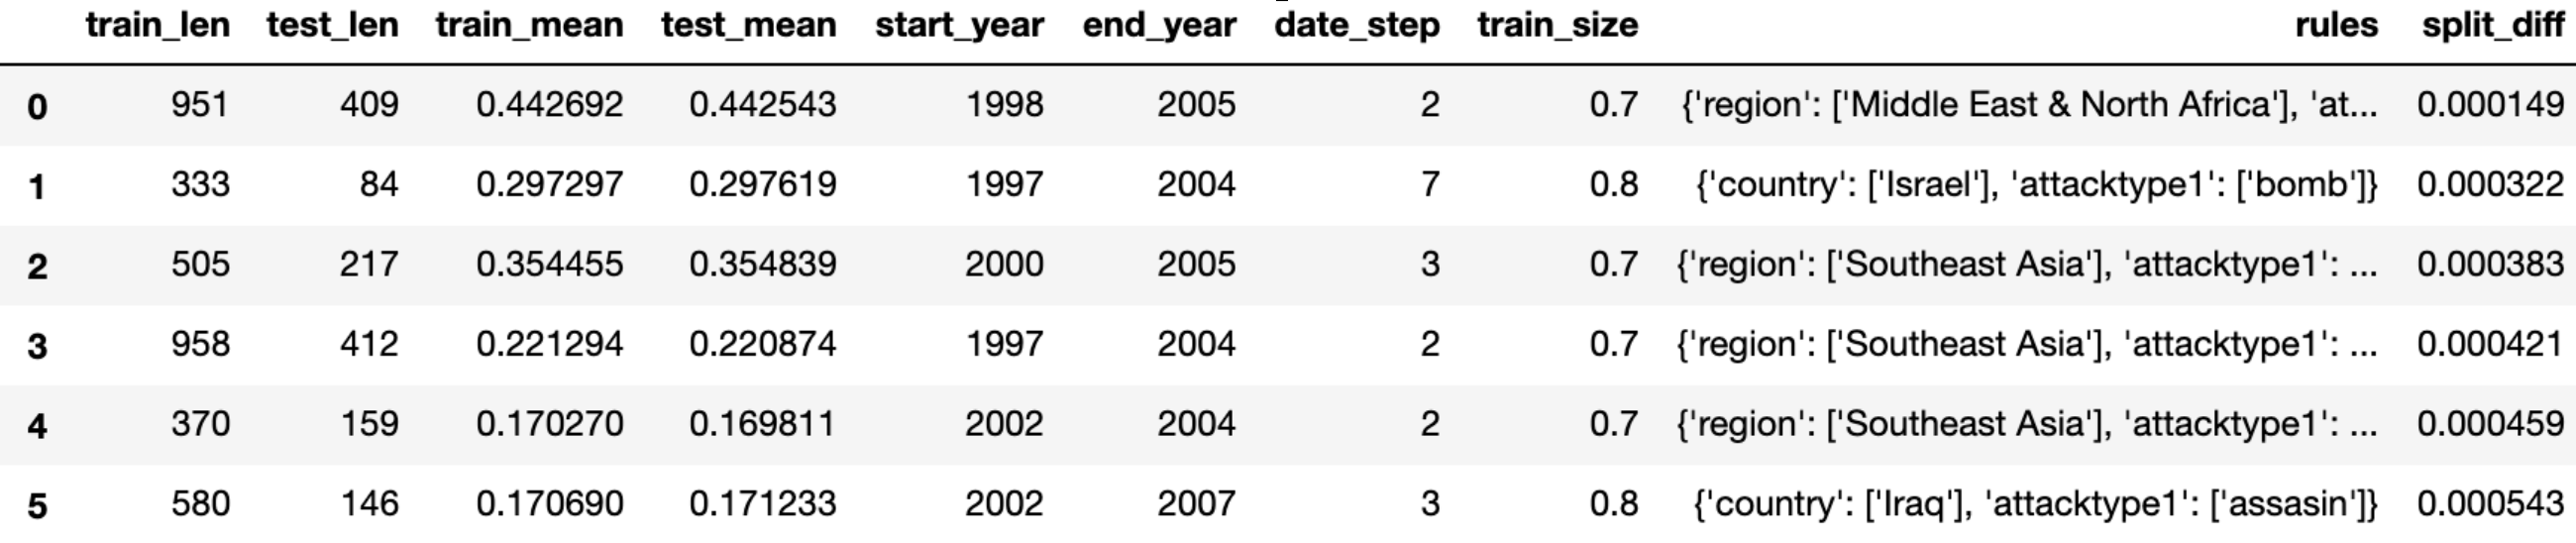
\includegraphics[width=\linewidth]{split_example.png}
%   \caption{Пример найденных разбиений для исходного набора данных}
%   \label{fig:split_example}
% \end{figure}

\subsubsection{Использование текстовых данных} \label{lda_topics}
% LDA model and document merging over agg period
В дополнение к существующим исходным признакам было решено использовать текстовые описания событий следующим образом:
\begin{enumerate}
    \item Для каждого агрегационного периода получить единственный текстовый документ путем склеивания всех текстовых описаний событий, входящих в период.
    \item Произвести классическую предобработку этих документов: удалить пунктуацию, нормализовать слов, удалить стоп-слова, ....
    \item Используя эти документы (точнее ту их часть, которая относится к тренировочной выборке) построить LDA-модель, т.е. построить распределение тематик по документам и распределение слов по тематикам для заданного количества тематик (в экспериментах количество тематик берется равным 10)
    \item Используя модель из предыдущего пункта получить 10 дополнительных признаков (соответствующих текстовым тематикам) для каждого агрегационного периода и использовать их вместе с признаками, соответствующими скрытому представлению.
\end{enumerate}
Поскольку получившаяся LDA-модель характеризует распределение слов по тематикам, ее можно применять для новых текстовых документов.
В частности, одно из текущих направлений - получить текстовые описания для всех событий из внешних источников, применить к ним обученную LDA модель и получить более точные тематические текстовые признаки.

Пример пяти тематик (их ключевых слов), выделенных с помощью LDA:
\begin{enumerate}
    \item incid bomb kill total relat
    \item claim respons group region kill
    \item group respons claim bomb injur
    \item incid target algerian take place
    \item algerian take place forc kill
\end{enumerate}

\begin{figure}
  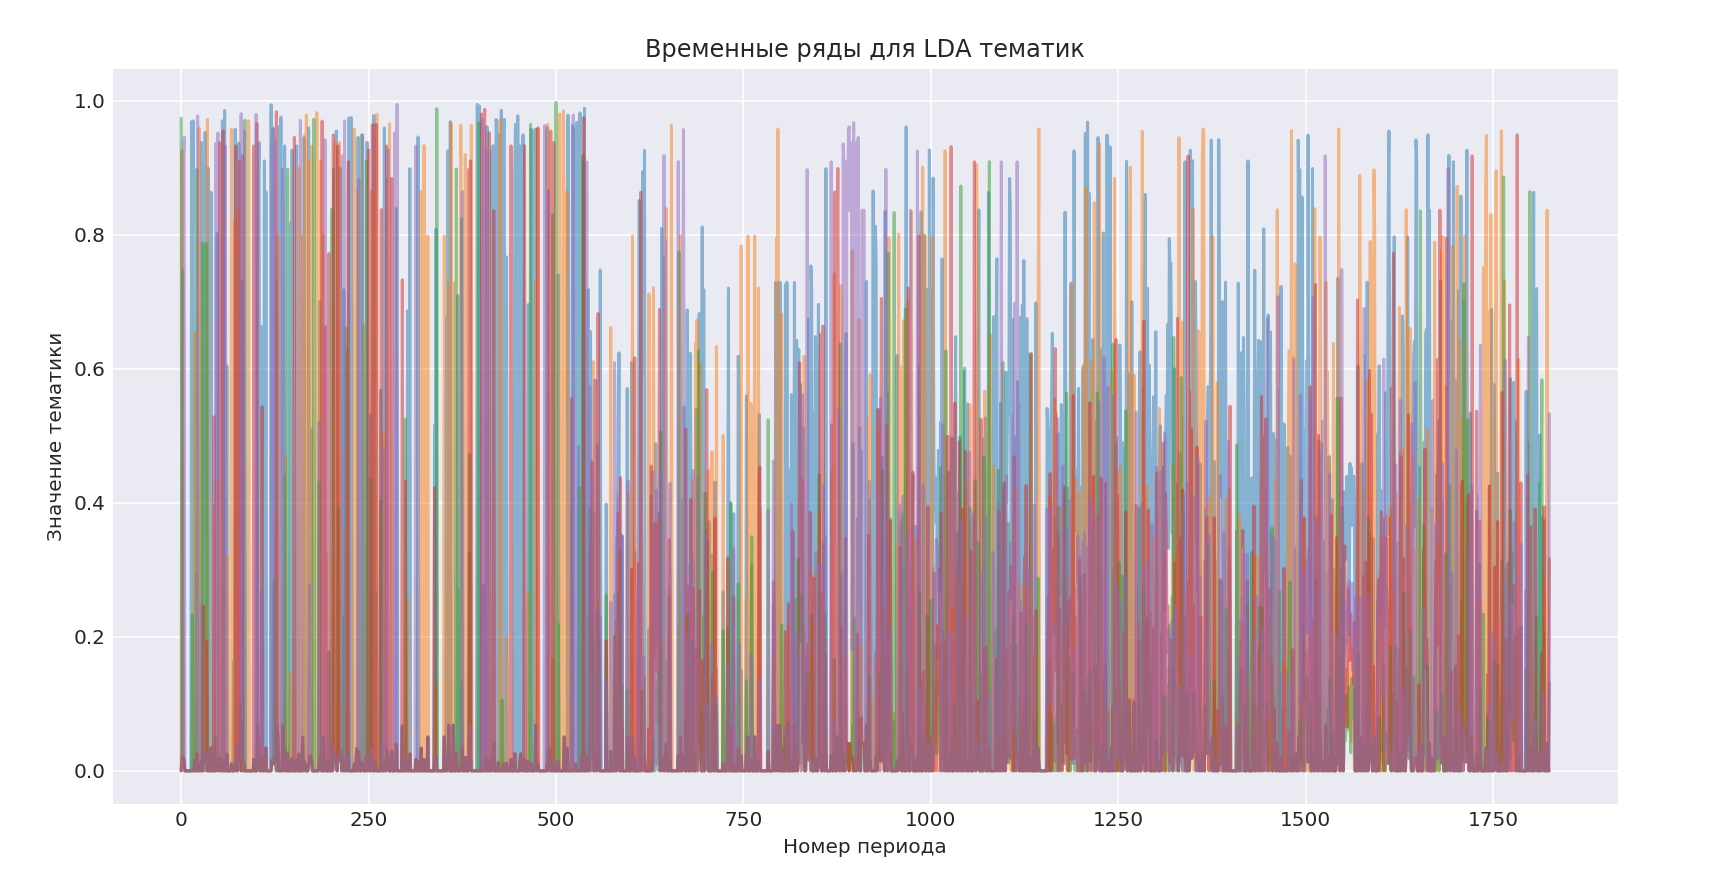
\includegraphics[width=\linewidth]{lda_example.png}
  \caption{Пример временных рядов для тематик LDA}
  \label{fig:lda_example}
\end{figure}

Пример соответствующих временных рядов можно увидеть на Рис. \ref{fig:lda_example}

\subsubsection{Результаты}
% Ниже приведены результаты для различных вариантов эксперимента.
Условия эксперимента:
\begin{enumerate}
    \item Год начала - 2002
    \item Год конца - 2008
    \item Длина агрегационного периода - 3 дня
    \item Тренировочная выборка: 70\%
    \item Целевые события: взрывы в Ираке (страна = Iraq, тип атаки = Bombing/Explosion)
\end{enumerate}
В рамках эксперимента были исследованы различные варианты представления событий -- с помощью NMF и с использованием автокодировщиков; количество тематик в экспериментах -- 10 и 50, так же вместе с тематиками были использованы дополнительные признаки AUX и REC.
В качестве моделей для прогнозирования были использованы классические модели классификации Logistic Regression (LogReg) и Random Forest Classifier (RFC), а так же нейронная сеть архитектуры LSTM.
Для задачи регрессии использовались модели Linear Regression (LinReg), Random Forest Regressor (RFR), а так же нейронная сеть архитектуры LSTM. Также варьировался размер окна исторических данных, которое мы принимали во внимание для построения прогноза. В текущем эксперименте были рассмотрены размеры окна равные 10 и 30.

В рамках экспериментов использовалась следующая архитектура сети LSTM: длина входной последовательности была равна 10 и 30 в зависимости от эксперимента и совпадала с размером окна исторических данных. Размерность скрытого слоя состояния LSTM-блока была равна размерности скрытого представления $k$ и принимала значения равные 10 и 50. При решении задачи прогнозирования вероятности события мы использовали функцию softmax для преобразования выхода сети в вероятности. В случае прогнозирования количества событий мы использовали линейную функцию активации. В процессе тренировки нейронной сети темп обучения был выбран равным $10^{-3}$, а количество эпох равным 50.

Обозначения:
\begin{itemize}
    \item  NMF\_N / AE\_N - использование тематик полученных с помощью NMF / Автокодировшика и с использованием N тематик
    \item + A - использование 2 дополнительных признаков (AUX), добавляющих авторегрессионную составляющую и описанных в \ref{train_process}
    \item + R - использование дополнительного признака, отвечающего за ошибку восстановления (реконструкции) в автокодировщике и описанного в \ref{train_process}
    %\item + text - использование 10 дополнительных тематик, описанных в \ref{lda_topics}
\end{itemize}

\subsubsection{Прогнозирование вероятности события}
Поскольку задача прогнозирования вероятности события сводится к задаче классификации и определения, произойдет событие или нет, для решения этой задачи были выбраны модели классификации.
В таблицах \ref{tab:clf-res-no-text} и \ref{tab:clf-res-text} представлены результаты решения задачи по метрике ROC AUC (чем меньше, тем лучше) для различных моделей и условий тестирования. Лучшие из обученных моделей смогли достигнуть ROC AUC $\approx$ 0.75-0.79. Лучшие результаты получали модели прогнозирования LSTM для всех трех вариантов извлечения этих тематик (матричная факторизация, автокодировщик, автокодировщик + ошибка восстановления). Также можно увидеть, что вспомогательные признаки (AUX) помогли моделям достигать более качественных результатов. Что касается размера окна (кол-ва исторических данных, использовавшихся для прогнозирования), то в среднем модели LSTM достаточно хорошо работали для размеров окна равных 10 и 30, в то время как классические модели (Random Forest Classifier, Logistic Regression) показывали более хорошие результаты на меньшем размере окна. Это может быть связанно с тем, что количество признаков при увеличении размера окна росло линейно и моделям было сложнее найти нужные паттерны в данных.
При использовании текстовых описаний модели LSTM показали как результатов, причем независимо от метода построения представления событий. Модели логистической регрессии и случайного леса на некоторых методах представления событий показали выигрыш по качеству с добавлением текстовых описаний, а на других стали работать немного хуже. Это, опять же, можно объяснить меньшей гибкостью линейных моделей и модели случайного леса.
\begin{center}
\begin{table}
 \begin{tabular}{||p{3.8cm}|p{1.5cm}|p{1.5cm}|p{1.5cm}|p{1.5cm}|p{1.5cm}|p{1.5cm}||} 
\hline
  & LSTM (L=10) & LSTM (L=30) & LogReg (L=10) & LogReg (L=30) & RFC (L=10) & RFC (L=30)\\ \hline\hline
AE\_10 & 0.616 & 0.641 & 0.439 & 0.417 & 0.484 & 0.509\\ \hline
AE\_10+A & 0.747 & 0.749 & 0.654 & 0.578 & 0.583 & 0.598\\ \hline
AE\_50 & 0.651 & 0.655 & 0.567 & 0.574 & 0.656 & 0.637\\ \hline
AE\_50+A & 0.743 & \textbf{0.752} & 0.655 & 0.552 & 0.658 & 0.578\\ \hline
AE\_10+R & 0.696 & 0.656 & 0.480 & 0.608 & 0.509 & 0.566\\ \hline
AE\_10+R+A & \textbf{0.764} & 0.744 & 0.653 & 0.572 & 0.609 & 0.615\\ \hline
AE\_50+R & 0.547 & 0.544 & 0.605 & 0.588 & 0.443 & 0.623\\ \hline
AE\_50+R+A & \textbf{0.761} & \textbf{0.760} & 0.655 & 0.551 & 0.659 & 0.606\\ \hline
NMF\_10 & 0.618 & 0.605 & 0.577 & 0.526 & 0.637 & 0.606\\ \hline
NMF\_10+A & 0.746 & 0.746 & 0.653 & 0.561 & 0.701 & 0.670\\ \hline
NMF\_50 & 0.691 & 0.711 & 0.537 & 0.446 & 0.650 & 0.533\\ \hline
NMF\_50+A & 0.740 & \textbf{0.783} & 0.658 & 0.580 & 0.638 & 0.671\\ \hline
 \end{tabular}
 \caption{\label{tab:clf-res-no-text} Результаты по метрике ROC AUC для задачи классификации без использования текста}
\end{table}
\end{center}

\begin{center}
\begin{table}
 \begin{tabular}{||p{3.8cm}|p{1.5cm}|p{1.5cm}|p{1.5cm}|p{1.5cm}|p{1.5cm}|p{1.5cm}||} 
\hline
& LSTM (L=10) & LSTM (L=30) & LogReg (L=10) & LogReg (L=30) & RFC (L=10) & RFC (L=30)\\ \hline\hline
AE\_10 & 0.597 & 0.657 & 0.505 & 0.563 & 0.679 & 0.361\\ \hline
AE\_10+A & \textbf{0.764} & 0.747 & 0.642 & 0.599 & 0.673 & 0.665\\ \hline
AE\_50 & 0.655 & 0.678 & 0.523 & 0.550 & 0.624 & 0.631\\ \hline
AE\_50+A & \textbf{0.752} & 0.745 & 0.645 & 0.493 & 0.681 & 0.614\\ \hline
AE\_10+R & 0.608 & 0.628 & 0.523 & 0.564 & 0.424 & 0.474\\ \hline
AE\_10+R+A & \textbf{0.795} & \textbf{0.758} & 0.642 & 0.576 & 0.644 & 0.619\\ \hline
AE\_50+R & 0.505 & 0.553 & 0.523 & 0.552 & 0.575 & 0.616\\ \hline
AE\_50+R+A & 0.736 & \textbf{0.759} & 0.644 & 0.523 & 0.674 & 0.504\\ \hline
NMF\_10 & 0.612 & 0.743 & 0.476 & 0.563 & 0.652 & 0.615\\ \hline
NMF\_10+A & 0.601 & \textbf{0.753} & 0.644 & 0.544 & 0.674 & 0.567\\ \hline
NMF\_50 & \textbf{0.776} & 0.688 & 0.484 & 0.547 & 0.575 & 0.498\\ \hline
NMF\_50+A & 0.741 & \textbf{0.753} & 0.645 & 0.569 & 0.688 & 0.625\\ \hline
 \end{tabular}
 \caption{\label{tab:clf-res-text} Результаты по метрике ROC AUC для задачи классификации с использованием текста}
\end{table}
\end{center}

\begin{figure}
  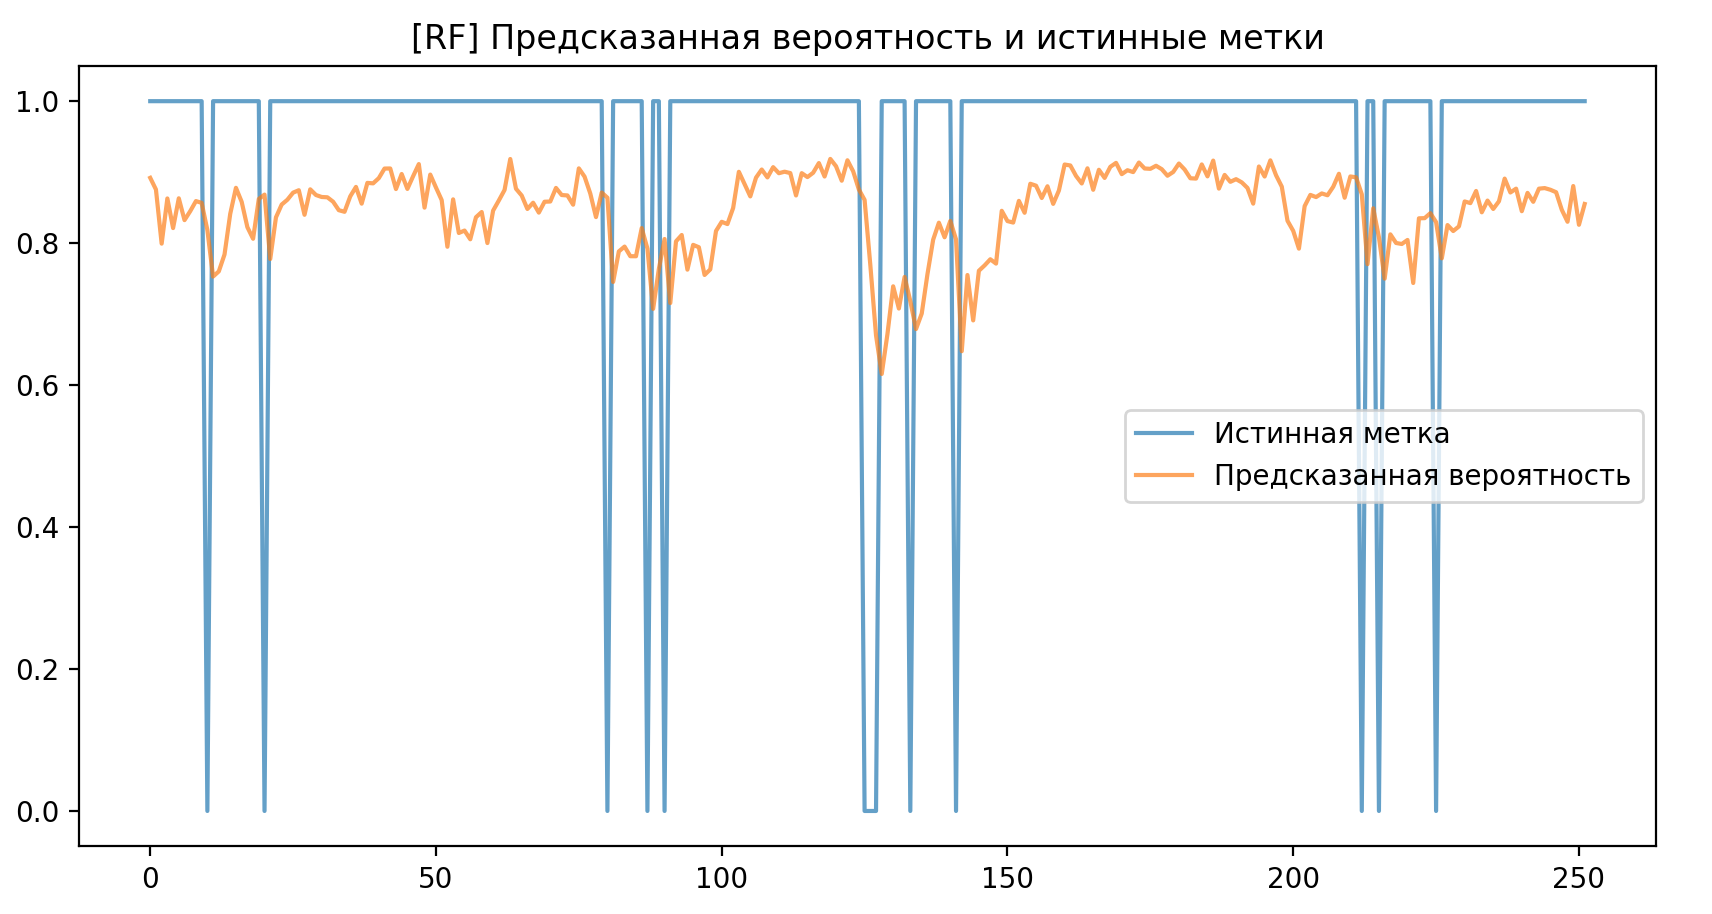
\includegraphics[width=\linewidth]{rf_clf_example.png}
  \caption{Пример работы модели классификации}
  \label{fig:rf_clf_example}
\end{figure}

\subsubsection{Прогнозирование количества событий}
Задача прогнозирования количества событий является задачей регрессии и может быть решена соответствующими моделями. В рамках экспериментов были рассмотрены модели линейной регрессии, случайного леса и нейросетевая модель архитектуры LSTM.
В таблицах \ref{tab:reg-res-no-text} и \ref{tab:reg-res} представлены результаты решения задачи регрессии по метрике MASE (чем меньше, тем лучше) для различных моделей и условий тестирования.

Исследовав распределение целевой переменной было решено попробовать предсказывать не количество $n$ событий, а величину $n' = log(1+n)$, восстанавливая затем $n$. Обозначим предсказанный логарифм как $y'$, а искомую величину за $y$. Тогда восстановить $y$ использую $y'$ можно следующим образом:
$$ y = e^{y' + \frac{\epsilon}{2}} - 1 $$
где $\epsilon$ - значение среднеквадратичной ошибки на специальной отложенной выборке.
Поскольку в этом случае требуется отложенная (валидационная) выборка, разбиение данных производится в пропорции 0.7 (тренировочная выборка) + 0.1 (валидационная) + 0.2 (тестовая). 

Лучше всех из регрессионных моделей себя показал случайный лес, стабильно достигая MASE = 0.9. Способ извлечения тематик, как оказалось, не играет решающей роли, как и количество интервалов, используемых для прогнозирования. Можно заметить, что дополнительные AUX-признаки значительно улучшают результаты, это вполне может быть вызвано тем, что они помогают модели случайного леса находить авторегрессионные зависимости, которые без этих дополнительных признаков найти было бы нетривиально. 
Какой-то сильной зависимости от использования или неиспользования текстовых признаков здесь обнаружить не удается, таким образом можно сделать вывод что решению задачи прогнозирования количества событий для рассмотренных моделей и методов построения представления использование текстовых признаков не помогает.
\begin{center}
\begin{table}
 \begin{tabular}{||p{3.8cm}|p{1.5cm}|p{1.5cm}|p{1.5cm}|p{1.5cm}|p{1.5cm}|p{1.5cm}||} 
\hline
& LSTM (L=10) & LSTM (L=30) & LinReg (L=10) & LinReg (L=30) & RFR (L=10) & RFR (L=30)\\ \hline\hline
AE\_10 & 1.218 & 1.204 & 1.119 & 1.191 & 1.241 & 1.265\\ \hline
AE\_10+A & 1.050 & 1.050 & \textbf{0.909} & 1.074 & \textbf{0.890} & \textbf{0.909}\\ \hline
AE\_10+R & 1.092 & 1.096 & 1.121 & 1.193 & 1.239 & 1.287\\ \hline
AE\_10+R+A & 1.054 & 1.072 & \textbf{0.911} & 1.102 & \textbf{0.886} & \textbf{0.910}\\ \hline
AE\_50 & 1.119 & 1.155 & 1.180 & 1.657 & 1.244 & 1.257\\ \hline
AE\_50+A & 1.084 & 1.055 & 1.632 & 1.616 & \textbf{0.883} & \textbf{0.904}\\ \hline
AE\_50+R & 1.040 & 1.039 & 1.209 & 1.580 & 1.243 & 1.278\\ \hline
AE\_50+R+A & 1.059 & 1.056 & 1.632 & 1.758 & \textbf{0.876} & \textbf{0.916}\\ \hline
NMF\_10 & 1.218 & 1.194 & 1.096 & 1.422 & 1.094 & 1.182\\ \hline
NMF\_10+A & 1.056 & 1.069 & \textbf{0.895} & 1.177 & \textbf{0.894} & \textbf{0.929}\\ \hline
NMF\_50 & 1.136 & 1.128 & 1.336 & 1.112 & 1.092 & 1.155\\ \hline
NMF\_50+A & 1.076 & 1.061 & 1.468 & 1.181 & \textbf{0.913} & \textbf{0.912}\\ \hline
  
\end{tabular}
\caption{\label{tab:reg-res-no-text} Результаты по метрике MASE для задачи регрессии без использования текста}
\end{table}
\end{center}

\begin{center}
\begin{table}
 \begin{tabular}{||p{3.8cm}|p{1.5cm}|p{1.5cm}|p{1.5cm}|p{1.5cm}|p{1.5cm}|p{1.5cm}||} 
\hline
& LSTM (L=10) & LSTM (L=30) & LinReg (L=10) & LinReg (L=30) & RFR (L=10) & RFR (L=30)\\ \hline\hline
AE\_10 & 1.104 & 1.151 & 1.292 & 2.151 & 1.295 & 1.323\\ \hline
AE\_10+A & 1.084 & 1.058 & 1.025 & 1.924 & \textbf{0.898} & \textbf{0.925}\\ \hline
AE\_10+R & 1.148 & 1.133 & 1.312 & 1.920 & 1.287 & 1.306\\ \hline
AE\_10+R+A & 1.047 & 1.067 & 1.029 & 1.745 & \textbf{0.896} & \textbf{0.929}\\ \hline
AE\_50 & 1.148 & 1.120 & 3.492 & 1.862 & 1.300 & 1.307\\ \hline
AE\_50+A & 1.046 & 1.068 & 3.082 & 1.810 & \textbf{0.899} & \textbf{0.918}\\ \hline
AE\_50+R & 1.124 & 1.136 & 2.840 & 1.967 & 1.305 & 1.307\\ \hline
AE\_50+R+A & 1.057 & 1.051 & 2.152 & 2.126 & \textbf{0.895} & \textbf{0.919}\\ \hline
NMF\_10 & 1.171 & 1.068 & 1.241 & 2.921 & 1.171 & 1.187\\ \hline
NMF\_10+A & 1.077 & 1.059 & \textbf{0.973} & 2.280 & \textbf{0.894} & \textbf{0.933}\\ \hline
NMF\_50 & 1.168 & 1.108 & 3.534 & 1.212 & 1.123 & 1.148\\ \hline
NMF\_50+A & 1.072 & 1.062 & 3.094 & 1.205 & \textbf{0.902} & \textbf{0.910}\\ \hline
\end{tabular}
\caption{\label{tab:reg-res} Результаты по метрике MASE для задачи регрессии c использованием текста}
\end{table}
\end{center}




\begin{figure}
  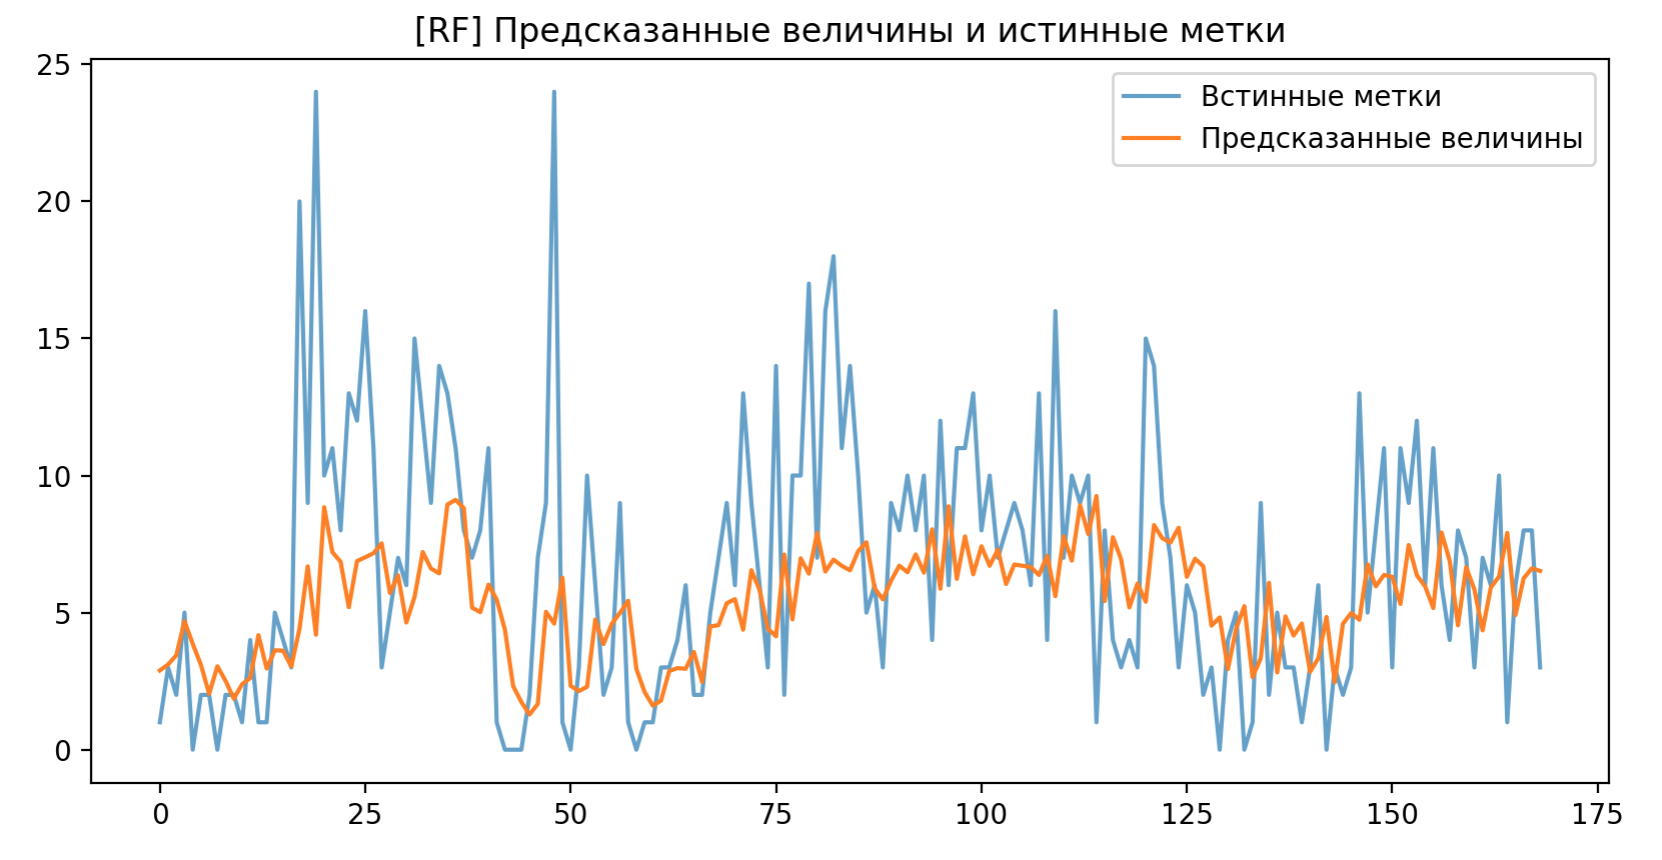
\includegraphics[width=\linewidth]{rf_reg_example.png}
  \caption{Пример работы модели регрессии}
  \label{fig:rf_reg_example}
\end{figure}

% \subsubsection{Регрессия логарифма целевой переменной}
% Исследовав распределение целевой переменной было решено попробовать предсказывать не количество $n$ событий, а величину $n' = log(1+n)$, восстанавливая затем $n$. Обозначим предсказанный логарифм как $y'$, а искомую величину за $y$. Тогда восстановить $y$ использую $y'$ можно следующим образом:
% $$ y = e^{y' + \frac{\epsilon}{2}} - 1 $$
% где $\epsilon$ - значение среднеквадратичной ошибки на специальной отложенной выборке.
% Поскольку в этом случае требуется отложенная (валидационная) выборка, разбиение данных производится в пропорции 0.7 (тренировочная выборка) + 0.1 (валидационная) + 0.2 (тестовая). 
% \par Ниже представлена метрика MASE (чем меньше, тем лучше) для различных моделей и условий тестирования. Метрика посчитана уже для восстановленных величин $y$.
% % description 
% % table
% \begin{center}
%  \begin{tabular}{||p{3.8cm}|p{1.5cm}|p{1.5cm}|p{1.5cm}|p{1.5cm}|p{1.5cm}|p{1.5cm}||} 
% \hline
%   & RFR (lag=10) & RFR (lag=30) &   LinReg (lag=10) & LinReg (lag=30) & LSTM (lag=10) & LSTM (lag=30)  \\ 
% \hline\hline
%  \hline
% \end{tabular}
% \end{center}
